\documentclass[a4paper]{scrartcl}                        % Blatt
\usepackage{amsmath,amsthm,amssymb,mathtools}
\usepackage{listings,physics}
\usepackage[left=2.5cm,right=2.5cm,top=2cm,bottom=1cm]{geometry}
%\usepackage[ngerman]{babel}
\usepackage{graphicx}
\usepackage{subcaption,siunitx,marvosym}
\usepackage{harpoon}
\usepackage[ngerman]{babel} 
\newcommand{\imu}{\mathrm{i}}

\newcommand{\vect}[1]{\overrightharp{\ensuremath{#1}}}
\newcommand{\field}[1]{\par\begin{large}{\vspace*{0.5cm}\noindent{}\textbf{#1}\vspace*{-1mm}}\end{large}}
\newcommand{\rom}[1]{\uppercase\expandafter{\romannumeral #1\relax}}
\sisetup{scientific-notation=engineering, exponent-product = \cdot, output-decimal-marker = {,}, separate-uncertainty, exponent-to-prefix}
%\newcommand{\problem}[2]{{\par\noindent{}\textit{Problem {\uppercase\expandafter{\romannumeral #1\relax}}.} #2}}
\newenvironment{problem}[3]{{\par\vspace*{4.5mm}\noindent{}\textit{Aufgabe {\uppercase\expandafter{\romannumeral #1\relax}}:} #2}\vspace*{+0.2cm}\hfill{\textit{
%#3
}}\\\hspace*{0.8cm}\hfill\begin{minipage}{\dimexpr\textwidth-1.3cm}}{\end{minipage}\hspace*{0.5cm}\\[.7em]}
\newenvironment{solution}[3]{{\par\vspace*{4.5mm}\noindent{}\textit{Lösung {\uppercase\expandafter{\romannumeral #1\relax}}:} #2}\vspace*{+0.2cm}\hfill{\textit{
%#3
}}\\\hspace*{0.8cm}\hfill\begin{minipage}{\dimexpr\textwidth-1.3cm}}{\end{minipage}\hspace*{0.5cm}\\[.7em]}
% don't fucking ask! (im 4h into this and it __works__)
% \vspace*{+0.2cm} -> \vspace*{-0.2cm} wenn die erste Zeile nen align is.

\begin{document}

\title{Übungsaufgaben komplexe Wechselstromrechnung}
\author{Kamal Abdellatif, Philip Geißler}
 
\maketitle

\field{Impendanz-, Strom, Spannungs-, Leistungs- und Arbeitsrechnung}
\begin{problem}{1}{Wirkleistung Motor}{placeholder}
Ein Elektromotor kann im Ersatzschaltbild als Reihenschaltung von einer Spule mit 
Induktivität $L_{\text{Motor}}$ und
eines Widerstandes $R_{\text{Motor}}$ dargestellt werden.
Der Motor habe \SI{1}{\kilo\watt} Wirkleistung bei $U_{\text{eff}} = \SI{230}{V}$ und $f = \SI{50}{\hertz}$.
Was ist die maximal mögliche Induktivität $L_{\text{Motor}}$ des Motors und welchen Widerstand $R_{\text{Motor}}$
würde dies erzwingen?
Vergleiche den Wirk- mit dem Blindwiderstand.
\end{problem}

\begin{solution}{1}{Wirkleistung Motor}{placeholder}
    \begin{align*}
        P_{\text{eff}} &= \frac{1}{2} \hat{U} \hat{I} \frac{\Re(R + X_L)}{\abs{R + X_L}} 
        = \frac{\hat{U}^2}{2}  \frac{\Re(R + X_L)}{\abs{R + X_L}^2} = \frac{\hat{U}^2}{2} \frac{R}{R^2 - X_L^2} \\
        R_{1/2} &= \frac{\hat{U}^2 \pm \sqrt{\hat{U}^4 + 16P_{\text{eff}}^2X_L^2}}{4P_{\text{eff} }}  
    \end{align*}
    Da $X_L^2$ negativ (oder 0) ist, gibt es 2 mögliche Motorwiderstände für geringe Induktivitäten.
    Für steigende Induktivitäten nähren sich diese aneinander an, bis sie bei der Grenzinduktivität denselben Wert wiedergeben. Für noch höhere Induktivitäten existieren keine Widerstände mehr, welche die angegebene Wirkleistung erzielen. Warum nicht?
    Um die Grenzinduktivität zu erhalten, setzen wir den Radikanten also gleich 0. 
    % i dont f***ing know :)
    \begin{align*}
         && 0 &\stackrel{!}{=} \hat{U}^4 + 16P_{\text{eff}}^2X_L^2 \\
         R_{1/2} &= \frac{\hat{U}^2 \pm \sqrt{0}}{4P_{\text{eff} }} = \frac{\hat{U}^2}{4 P_{\text{eff}}}
         &   \implies X_L &= \frac{\hat{U}^2}{4 P_{\text{eff}}}\imu = R_{1/2} \imu
    \end{align*}
    Im Grenzfall sind Blind- und Wirkwiderstand also gleich.
    Nun können wir schließlich noch den Spezialfall explizit ausrechnen.
    \begin{align*}
        R_{\text{Motor}} &= \frac{\hat{U}^2}{4 P_{\text{eff}}} 
            = \frac{(\sqrt{2}\cdot \SI{230}{\volt})^2}{\SI{4}{\kilo\watt}} = \SI{26.45}{\ohm}\\
        L_{\text{Motor}} &= \frac{X_L}{\omega\imu } = \frac{R_{\text{Motor}}\imu }{ 2 \pi \imu f}
            = \frac{\SI{26.45}{\ohm}}{ 2 \pi \cdot  \SI{50}{\hertz}} \approx \SI{84.2}{\milli\henry}
    \end{align*}
\end{solution}

\newpage

\begin{problem}{2}{Motorkompensation}{placeholder}
Selbes Motorkonzept, anderer Motor.
Der Wirkwiderstand $R_{\text{Motor}}$ sei $\SI{10}{\ohm}$.
Man habe nun die Möglichkeit, ein weiteres passives Bauteil parallel zum Motor zu schalten, um die Blindleistung 
der Gesamtschaltung zu minimieren. Welches Bauteil sollte man wählen und wie verhält sich dessen Kenngröße in Abhängigkeit von $L_{\text{Motor}}$.
Man berechne die Kenngröße explizit für $L_{\text{Motor}} = \SI{0.1}{\henry}$ und $f = \SI{50}{\hertz}$.
\end{problem}

\begin{solution}{2}{Motorkompensation}{placeholder}
    \begin{minipage}{0.6\textwidth}
        \begin{align*}
            X_{R,L} &= R + \imu \omega L \\
            Z &= X_{R,L} \parallel X_X = \frac{1}{\frac{1}{R + \imu \omega L} + \frac{1}{X_X}} 
        \end{align*}
    \end{minipage}
    \begin{minipage}{0.03\textwidth}
        ~~~~~
    \end{minipage}
    \begin{minipage}{0.3\textwidth}
        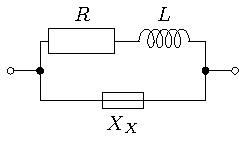
\includegraphics[width=\textwidth]{loes2.pdf}
    \end{minipage}\\[.3em]
    Wir können versuchen, den Gesamtblindwiderstand gleich 0 zu setzen.
    Denn sollte dies möglich sein, so haben wir mit Sicherheit den Blindwiderstand minimiert.
    \begin{align*}
        \Re(Z) = Z &= \frac{1}{\frac{1}{R + \imu \omega L} + \frac{1}{X_X}}
        = \frac{1}{\frac{X_X + R + \imu \omega L}{X_X \cdot (R + \imu \omega L)}}
        = \frac{X_X \cdot (R + \imu \omega L)}{X_X + R + \imu \omega L}
    \end{align*}
    Hier ergibt sich die triviale Lösung, $X_X = \SI{0}{\ohm}$ zu setzen. Dies entspricht aber einer Parallelschaltung mit einem Kurzschluss, über welchen logischerweise jeder Strom fließt (keine Resonanz). Da der Motor dadurch aber nutzlos wird, schließen wir diese Lösung aus und bringen den Bruch auf einen reellen Nenner.
    \begin{align*}
        \frac{ \imu \omega L X_X + R X_X}{R + (\imu \omega L + X_X)} 
            &= \underbrace{\frac{\imu \omega L X_X R - \imu \omega L R X_X - R X_X^2}{R^2 - (\imu \omega L + X_X)^2}}_{\text{Realteil}}
            + \underbrace{\frac{R^2 X_X  + \omega^2 L^2 X_X - \imu \omega L X_X^2}{R^2 - (\imu \omega L + X_X)^2}}_{\text{Imaginärteil (reeller Nenner)}} \\
            \implies \qquad\qquad 0 &= R^2 X_X  + \omega^2 L^2 X_X - \imu \omega L X_X^2 \\
            \omega L \cdot X_X \imu &= R^2 + \omega^2L^2\\
            X_X &= -\frac{R^2 + \omega^2L^2}{\omega L}\imu \quad \implies \quad \Im(X_X) < \SI{0}{\ohm}
    \end{align*}
    Das kompensierende Bauteil sollte also kapazitiv sein. Einsetzen der vorgegebenen Größen liefert
    \begin{align*}
        X_C &= -\frac{(\SI{10}{\ohm})^2 + (2\pi \cdot \SI{50}{\hertz})^2
        (\SI{0.1}{\henry})^2}{2\pi\cdot  \SI{50}{\hertz}\cdot \SI{0.1}{\henry}}\imu
        \approx -{34.6 \imu}\si{\ohm}\\
        C &= \frac{-\imu}{\omega X_C} = \frac{1}{2\pi\cdot \SI{50}{\hertz} \cdot \SI{34.6}{\ohm}} 
        \approx \SI{9.2e-5}{\farad}
    \end{align*}
\end{solution}

\newpage

\begin{problem}{3}{Kenngrößen des kompensierten $RC$-Spannungsteilers}{placeholder}
    \begin{minipage}{0.55\textwidth}
        Ein Spannungsteiler aus zwei Widerständen mit den Widerstandswerten $R_1$ und $R_2$ wird mit
        einem Kondensator $C_L$ im Wechselstrom belastet. Zu diesem Zeitpunkt sei die Kapazität $C_R$ des Regelkondensators noch 0, praktisch ein offener Schalter.
        Wie sehr bricht die Ausgangsspannung in Abhängigkeit der Kreisfrequenz ein [$f(\omega) \coloneqq U_a(\omega)/{U_e}$]?\\[-.73em]
    \end{minipage}
    \begin{minipage}{0.03\textwidth}
        ~~~~~
    \end{minipage}
    \begin{minipage}{0.4\textwidth}
        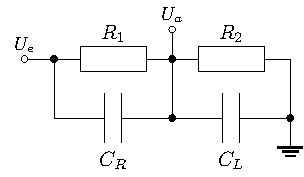
\includegraphics[width=\textwidth]{aufg3.pdf}
    \end{minipage}
    Welches Verhalten lässt sich beobachten, wenn man nun $C_R$ so auswählt, dass $C_RR_1 = C_LR_2$ gilt?
\end{problem}

\begin{solution}{3}{Kenngrößen des kompensierten $RC$-Spannungsteilers}{placeholder}
    Die Gesamtschaltung bleibt weiterhin ein Spannungsteiler, nur nun mit einer Parallelschaltung aus Kondensator und Widerstand. Insofern kann man die übliche Spannungsteilerformel verwenden.
    \begin{align*}
        U_a &= \frac{R_2 \parallel X_{C_L}}{R_1 + (R_2 \parallel X_{C_L})} & R_2 \parallel X_{C_L} 
            = \frac{R_2\cdot X_{C_L}}{R_2 +     X_{C_L}}
    \end{align*}
    Definieren wir uns nun die normierte Frequenz $\Omega_L = \omega R_2C_L$, so können wir uns die Ausgangsspannung in einigen Grenzfällen für $\omega$ approximieren, um ein Gefühl für das Verhalten der Übertragsfunktion zu bekommen.
    \begin{align*}
        R_2 \parallel X_{C_L} &= \frac{\frac{R_2}{\imu \omega C_L}}{R_2 + \frac{1}{\imu \omega C_L}}
        = \frac{R_2}{1 + \imu \Omega_L} \approx \begin{cases}
             R_2 & \text{für } \Omega_L \ll 1 \\ 
             \frac{R_2}{1 + \imu} & \text{für } \Omega_L = 1 \\
             X_{C_L} & \text{für } \Omega_L \gg 1 
        \end{cases} \\
        \implies  \frac{U_e}{U_a} &\approx \begin{cases}
            \frac{R_2}{R_1 + R_2} & \text{für } \Omega_L \ll 1 \\ 
            \frac{R_2}{(1 + \imu)R_1 + R_2} & \text{für } \Omega_L = 1 \\
            \frac{X_{C_L}}{R_1 + X_{C_L}} & \text{für } \Omega_L \gg 1 
        \end{cases}  
    \end{align*}
    Für niedrige Frequenzen arbeitet der kapazitive Spannungsteiler wie ein ohmscher, für große Frequenzen 
    $\omega^{-1} \ll R_2C_L$ sinkt die Ausgangsspannung wie beim Tiefpass 1.Ordnung, mit der Grenzkreisfrequenz $(R_2C_L)^{-1}$.
    Setzen wir nun $C_RR_1 = C_LR_2$, so wird auch die erste Teilimpedanz des Spannungsteilers komplex. Wir definieren zusätzlich noch $\Omega_R = \omega R_1C_R$ zur Vereinfachung der folgenden Formeln und bemerken $\Omega_L = \Omega_R \eqqcolon \Omega$.
    \begin{align*}
        \frac{U_e}{U_a} &= \frac{R_2 \parallel X_{C_L}}{(R_1 \parallel X_{C_R}) + (R_2 \parallel X_{C_L})}
            = \frac{\frac{R_2}{1+\imu \Omega_L}}{\frac{R_1}{1 + \imu \Omega_R} + \frac{R_2}{1+\imu \Omega_L}} \\[.2em]
        &= \frac{(1 + \imu \Omega_R)R_2}{(1 + \imu \Omega_L)R_1 + (1 + \imu \Omega_R)R_2}
        = \frac{(1 + \imu \Omega)R_2}{(R_1 + R_2) + (R_1+ R_2)\Omega\imu} \\[.2em]
        &= \frac{R_2}{R_1 +R_2} \cdot \frac{1 + \Omega\imu}{1 + \Omega\imu} = \frac{R_2}{R_1 +R_2}
    \end{align*} 
    Für ein solches Verhältnis der Kapazitäten und Widerstände ist das Spannungsteilerverhältnis also 
    unabhängig von der Frequenz des Signals.
    Dies wird sich bei Tastköpfen von Oszilloskopen zunutze gemacht, da die Eingänge sowohl Widerstand als auch Kapazität aufweisen. Tastköpfe haben dies dann auch (mit einstellbarer Kapazität) und werden dann vor das Oszilloskop, sodass der Eingang hochfrequente nicht stärker als niederfrequente Signale dämpft, wie es beim Frequenzunkompensierten Spannungsteiler (erster Aufgabenteil) der Fall wäre. 
\end{solution}


\begin{problem}{4}{Leistungskosten}{placeholder}
    Energieversorger rechnen für Privatkunden Blind- und Wirkleistung nicht getrennt ab.
    Stattdessen wird von einer ohmschen Belastung ausgegangen und Energie ($p = 31,\!5\text{ct}/\text{kWh}$) über die approximierte Leistung $\tilde{P} = U_{\text{eff}}I_{\text{eff}}$ berechnet.
    Angenommen man hat in seiner Wohnung $R_{\text{Last}}=\SI{100}{\ohm}$ einen Kondensatorschrank $C = \SI{1}{\farad}$ parallel angeschlossen. Wie viel zahlt man dann jährlich zu viel an den Energieversorger? (Annahme: Blindleistung eigentlich kostenlos, da keine Energie verloren geht.)
\end{problem}

\begin{solution}{4}{Leistungskosten}{placeholder}
    Über die Impedanz erhält man sowohl die Effektive Leistung, als auch den Scheinwiderstand, aus welchem man die Scheinleistung erhält.
    Diese muss man dann nur noch mit der Zeit und dem Preis multiplizieren um die jährlichen Kosten zu erhalten.
    \begin{align*}
        Z &= R \parallel X_C = \frac{1}{\frac{1}{\SI{100}{\ohm}} + \imu 2 \pi \cdot \SI{50}{\hertz}} 
        \approx (10^{-6}-3\cdot10^{-3}\imu)\si{\ohm}\\
        P_{\text{eff}} &= \frac{\hat{U}\hat{I}}{2} \frac{\Re(Z)}{|Z|} = U_{\text{eff}}^2 \frac{\Re(Z)}{|Z|^2}
        \approx \SI{5290}{\watt} & \mathllap{\text{Wirkleistung}} \\
        \tilde{P} &= U_{\text{eff}}I_{\text{eff}} = U_{\text{eff}}^2 \frac{1}{|Z|} 
        = P_{\text{eff}} \frac{|Z|}{\Re(Z)} \approx \SI{16.62}{\mega\watt} & \mathllap{\text{Scheinleistung}} \\
        \text{jährl. Kosten} &= \tilde{P}\cdot T \cdot p 
        = \SI{16.62}{\mega\watt} \cdot \SI{31.54}{\mega\second} \cdot 31,\!5\text{ct}/\text{kWh} \approx 45,\!86\,\text{Mio.\EURtm}\\
        \text{Extrakosten} &= (\tilde{P}-P_{\text{eff}})\cdot T \cdot p 
        = \SI{16.61}{\mega\watt} \cdot \SI{31.54}{\mega\second} \cdot 31,\!5\text{ct}/\text{kWh} \approx 45,\!85\,\text{Mio.\EURtm}
    \end{align*}
    Ganz schön teuer. 
\end{solution}

\newpage

\field{Konzeption komplexer Wechselstrom}
\begin{problem}{1}{Effektive und Exakte verrichtete Arbeit}{placeholder}
Ab welcher Länge eines $\SI{1}{\mega\hertz}$ Signales über ein $RC$-Reihenglied (\SI{100}{\ohm}, \SI{10}{\nano\farad}) weicht die effektive Arbeit nur noch maximal ein Promille von der exakten Arbeit ab?
% Das is nich mal __genau__ genau, sondern nur grob genau
% genau genau is sowiso prbly nur numerisch machbar.
\end{problem}



\begin{solution}{1}{Effektive und Exakte verrichtete Arbeit}{placeholder}
    Berechnen wir die Impedanz des Reihengliedes, so können wir aus dieser auf die exakte und effektive Leistung 
    schließen und daraus dann die Arbeit erhalten.
    $$X = (100 - 100\imu)\si{\ohm}\hspace*{4cm}$$\\[-3.5em]
    \begin{align*}
        P_{\text{eff}} &= \frac{1}{\sqrt{2} \cdot 2}\cdot \hat{U} \hat{I} &
        P_{\text{exakt}} &= \sin(2\pi \cdot \SI{1}{\mega\hertz}) \cdot \sin(2\pi \cdot \SI{1}{\mega\hertz} + \frac{\pi}{4}) \cdot \hat{U} \hat{I} \\
        W_{\text{eff}} &= P_{\text{eff}}\hspace*{.3mm}t = \frac{\hat{U} \hat{I}}{\sqrt{2} \cdot 2} t &    
        W_{\text{exakt}} &= \frac{\hat{U} \hat{I} \cdot t}{\sqrt{2} \cdot 2} - \frac{\cos(\SI{4}{\mega\hertz} \cdot \pi t) + \sin(\SI{4}{\mega\hertz} \cdot \pi t)}{\sqrt{2}\pi \cdot \SI{8}{\mega\hertz} } \cdot \hat{U} \hat{I} \\
    \end{align*}\\[-3.5em]
    \begin{align*}
        \frac{W_{\text{eff}} - W_{\text{exakt}}}{W_{\text{eff}}} &= 
        \frac{\cos(\SI{4}{\mega\hertz} \cdot \pi t) + \sin(\SI{4}{\mega\hertz} \cdot \pi t)}{\sqrt{2}\pi \cdot \SI{8}{\mega\hertz}} \frac{\sqrt{2} \cdot 2}{t}= 
        \frac{\sin(\frac{\pi}{4} + \SI{4}{\mega\hertz} \cdot \pi t)}{\sqrt{2}\pi t \cdot \SI{2}{\mega\hertz}} \\
        &\leq \frac{1}{\sqrt{2}\pi t \cdot \SI{2}{\mega\hertz}} \stackrel{!}{=} \frac{1}{1000} \\
        &\hspace*{1.018cm}\implies t_{\text{Abw}} \approx \frac{1000}{\sqrt{2}\pi \cdot \SI{2}{\mega\hertz}}  
        =\frac{\SI{1}{\milli\second}}{2\sqrt{2}\pi} \approx \SI{113}{\micro\second}
    \end{align*}
    Man sieht, dass die effektive Arbeit bei solchen Frequenzen sehr schnell sehr genau der exakten Arbeit entspricht und sich immer weiter mit $1/t$ relativ gegen die exakte Arbeit annähert.
    Was gegebenenfalls auffällt, ist dass die exakte Leistung zwischenzeitlich negativ ist. Dies lässt sich dadurch erklären, dass die Schaltung die vorher elektrisch gespeicherte Arbeit (von dann, wenn $P_{\text{exakt}} > P_{\text{eff}}$) wieder abgibt, und damit insgesamt kurzzeitig Energie abgibt.
\end{solution}

\newpage

\begin{problem}{2}{Nichtnegativer Wirkwiderstand}{placeholder}
Jedes einzelne passive Bauteil hat einen nichtnegativen Wirkwiderstand.
Aus der Abgeschlossenheit der komplexen Zahlen unter Addition und Inversion folgt, dass auch 
Kombinationen von Reihen- und Parallelschaltungen nichtnegative Wirkwiderstände besitzen, 
da die Gesamtimpedanz von diesen nur durch
Inversion und Addition aus den Einzelimpedanzen berechnet werden kann. ($R$ Sei der Wirkwiderstandsteil und $K$ der komplexe Teil der Impedanz.)
\begin{align*}
    Z_1 + Z_2 &= (R_1+R_2) + (K_1 + K_2)\imu 
    &\implies&& \Re(Z_1 + Z_2) &= R_1+R_2 \geqslant 0\\
    \frac{1}{Z_1} &= \frac{R_1-I_1\imu}{R_1^2 + K_1^2}
    &\implies&& \Re\qty(\frac{1}{Z_1}) &= \frac{R_1}{R_1^2 + K_1^2} \geqslant 0
\end{align*}
Man beweise, ob/dass dies auch für allgemeine Zweipolschaltungen (wie z.b. die H-Brücke) gilt.
\end{problem}

%
% I dont have no solution :/
%

\end{document}
